\chapter{Results and Discussion}\label{ch:results}

Due to limit of time and equipment, the analysis and results are based on set of test 1. The equipment and running procedures are demostrated in Chapter 3. The analysis results and detail discussion is included in this part. In the next semester, data from other two tests will be investigated.

\section{Resonance Compensation}

The cepstrum modification method is performed to compensate the amplitude modulation caused by resonance. Firstly, perform invers Fourier transform on the log spectrum of the external vibration signal to get the cepstrum. It is presented in Figure 4.1 (1). Gao and Randall indicated in \cite{Gao1} \cite{Gao2} that the modal information tend to locate at the low quefrency range and thus could be extracted by a 'shortpass lifter'. In this project, a decaying exponentila lifter is utilized. The cepstrum before and after liftering is shown in Figure 4.1.

\begin{figure}[h]
	\centering
	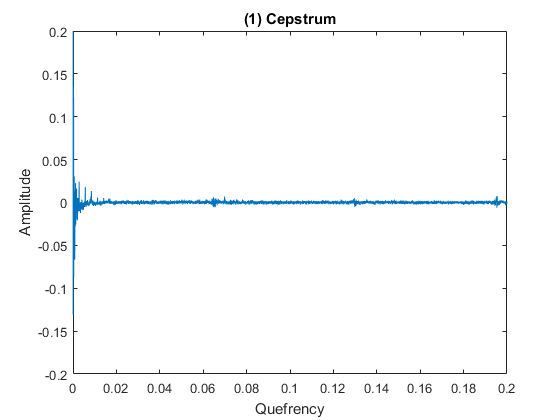
\includegraphics[scale =0.48]{cepstrum}
	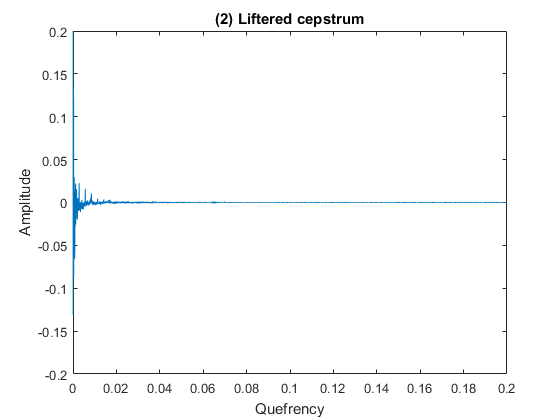
\includegraphics[scale =0.48]{lifteredCepstrum}
	\caption{Cepstrum before and after exponential liftering}
	\label{cepstrum}
\end{figure}

Comparing the orignal and liftered cepstrum, the high quenfrency signals are canceled out. Those signals tend to contain the harmonic and sideband information in order domain. The liftered cepstrum is Fourier transformed and exponentialed to get the modal spectrum. The original spectrum and the modal spectrum is shown in Figure 4.2 (1). The original sigal is in red and the modal is the black curve.

The modal information is anticipated to contain the amplitude modulation effect caused by frequency response fuction. Thus substracting modal from original frequency is able to compensate the resonance. The modified spectrum is shown in Figure 4.2 (2). The residual spectrum is smooth and uniform in amplitude.


\begin{figure}[h]
	\centering
	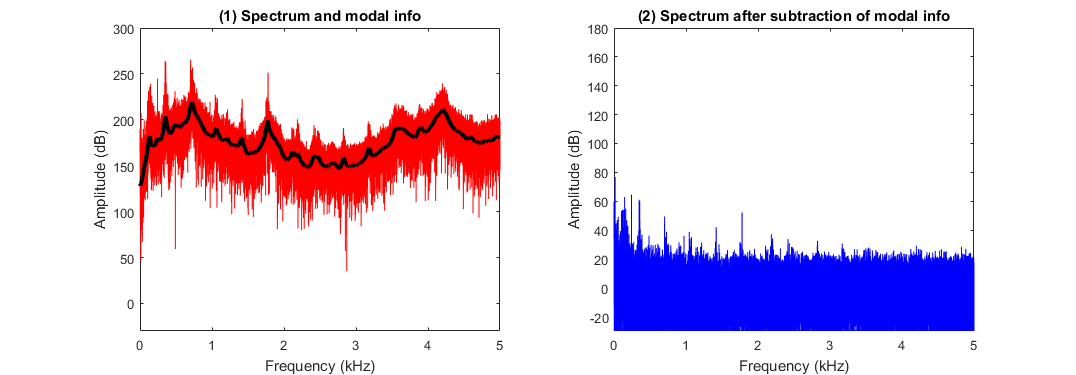
\includegraphics[scale =0.5]{composant}
	\caption{Spectrum before and after substraction of modal information}
	\label{composant}
\end{figure}

\section{Order Tracking and Hilbert Transform}

The order tracking process is to resample the vibration signal in equal phase difference. The phase-fixed tacho signal is use as reference. A new sample rate of how many samples per one revolution should be defined.
The horizontal axis of order tracked signal is orders. It is transfered from input shaft to the carrier speed in process. So the planet carrier frequency is 1 Hz. The frequencies of each part of the planetary gearbox is calculated as:

\begin{table}[h]
	\centering
	\caption{Frequency of each part}
	\label{gear frequencies}
	\begin{tabular}{p{80pt}p{80pt}p{80pt}}
		\toprule
		\textbf{Part} & \textbf{Teeth number} & \textbf{Frequency} \\ 
		\midrule
		Carrier & 55  & 1\\
		Pinon   & 42  & 1.31\\
		Planet  & 23  & -2.48\\
		Ring    & 80  & 0\\
		Sun     & 34  & 3.35\\
		\bottomrule
	\end{tabular}
\end{table}

Among these parts of the planetary gearbox, the frequency of the planet gear is negtive, which means the running direction of the planet gear is oposite with the others. In addition, based on the tooth numbers and running speed data, the gear mesh frequency of the pinon and spur gears could be calculated as $fc * Nc = 55 Hz$, while that of the planetary gearbox is $fc * Nr = 80 Hz$.

The order tracked signal is now constant in speed. Hilbert transform is now performed to extract the modulation signal. This is actually delay the phase of the orignal signal 90 digrees to form the imaginary part, and then combine with the original real part to become a analytic signal. The amplitude of the analytic signal is now the amplitude modification signal. While its phase deviation reveals the frequency modulation signal. The impulses caused by gear fault would mainly have effect on the amplitude of vibration. The phase modulation is unconspicuous. Thus only amplitude demodulation is performed in the Hilbert transform process.

The demodulated signal was Fourier transformed to obtain its spectrum, which is shown below in Figure 4.3. In this plot, 3.48 Hz and its harmonics are clearly revealed. As is known, the planet gears in the planetary gearbox not only spin around their own axle but also turn around the sun gear together with the planet carrier. Thus the fault frequency of the planet gears is $2.48 + 1 = 3.48 Hz$, which is exactly what is got in the plot.

\begin{figure}[h]
	\centering
	\includegraphics[scale =0.8]{hilbert}
	\caption{Spectrum after Hilbert transform}
	\label{hilbert}
\end{figure}


\section{Discussion}

The results shows this diagnosis procedure is able to work out the fault information. But the speed variation of data from test 1 is slow and narrow. No obvious resonance effect is able to be seen. One possible appearance is seen around 10 secends. Seen from Figure 4.5, the speed then is about 8 Hz on the VFD and 2 Hz for the input shaft. This 5s to 15s signal is seperated for detail investigation. 

\begin{figure}[h]
	\centering
	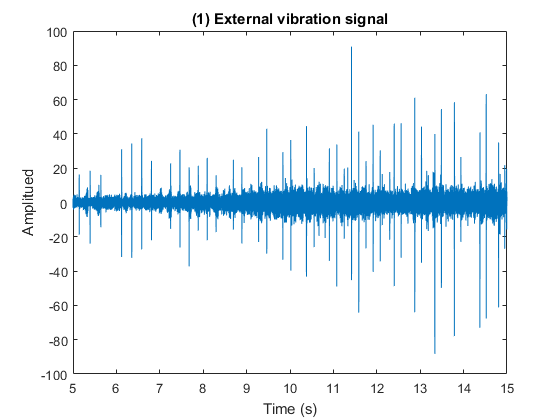
\includegraphics[scale =0.48]{5t15}
	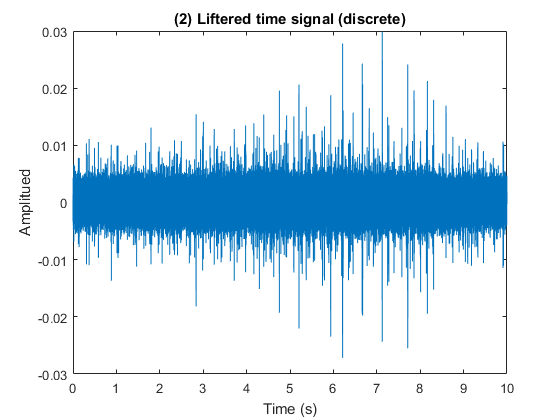
\includegraphics[scale =0.48]{5t15lift}
	\caption{Waveform of 5s to 15s before and after cepstrum modification}
	\label{5to15}
\end{figure}

Seen from Figure 4.4, the cepstrum modification performance is effective to compensate the suspect resonance around 10 second. But the diagnosis result is not as obvious as in Figure 4.3. Which means the exponential liftering not only canceled the modal information but also affected the impulses produced by gear fault. Other liftering width and methods will be compared in the following test.






